%% LyX 2.3.6.1 created this file.  For more info, see http://www.lyx.org/.
%% Do not edit unless you really know what you are doing.
\documentclass[english]{article}
\usepackage[T1]{fontenc}
\usepackage[latin9]{inputenc}
\usepackage{geometry}
\geometry{verbose,tmargin=2.5cm,bmargin=2.5cm,lmargin=2.5cm,rmargin=2.5cm}
\usepackage{calc}
\usepackage{textcomp}
\usepackage{graphicx}
\PassOptionsToPackage{normalem}{ulem}
\usepackage{ulem}

\makeatletter

%%%%%%%%%%%%%%%%%%%%%%%%%%%%%% LyX specific LaTeX commands.
%% Because html converters don't know tabularnewline
\providecommand{\tabularnewline}{\\}

\makeatother

\usepackage{babel}
\begin{document}
{[}SPLIT\_HERE{]}
\begin{enumerate}
\item \textbf{{[}PJC/PRELIM/9597/2018/P1/Q1{]} }

You are provided with the usernames and passwords of some members
of a recreation club in the text file \texttt{ACCOUNTS.txt}. The format
of each record is: 
\noindent \begin{center}
\texttt{<username> <password> }
\par\end{center}

Sample records from the file:

\noindent %
\noindent\begin{minipage}[t]{1\columnwidth}%
\texttt{bzkoh F9obSbf2\&}

\texttt{pdnathan \%57+g/J{[} }%
\end{minipage}

Members use their usernames and passwords to login to the club\textquoteright s
portal to book facilities. Arising from a new IT security policy,
all passwords must fulfil all the following requirements: 
\begin{itemize}
\item At least 8 characters in length, 
\item At least 1 uppercase letter, 
\item At least 1 lowercase letter, 
\item At least 1 digit, 
\item At least 1 punctuation mark / special symbol which is a printable
ASCII character (excluding whitespace). 
\end{itemize}
These characters have ASCII code (in decimal) from
\begin{itemize}
\item 33 to 47
\item 58 to 64 
\item 91 to 96
\item 123 to 126 
\end{itemize}
For examples, ASCII code 33 is \textquoteleft \texttt{!}\textquoteright ,
ASCII code 47 is \textquoteleft \texttt{/}\textquoteright{}

\textbf{Examples of passwords that fulfil all requirements:}
\noindent \begin{center}
\begin{tabular}{|c|c|c|c|}
\hline 
\texttt{AbCd35{*}n} & \texttt{iloveApples2\textbackslash} & \texttt{3\#\$\%\textasciicircum\&{*}(Kc} & \texttt{<jumping9Jac>}\tabularnewline
\hline 
\end{tabular}
\par\end{center}

\textbf{Examples of passwords that do not meet all requirements and
reasons: }
\noindent \begin{center}
\begin{tabular}{|c|c|}
\hline 
\texttt{cocoN8\%} & Less than 8 characters.\tabularnewline
\hline 
\texttt{coconut8\%} & No uppercase letter.\tabularnewline
\hline 
\texttt{COCO8888} & No lowercase letter. No symbol\tabularnewline
\hline 
\texttt{iLikeDo\textasciicircum{} } & No digit. \tabularnewline
\hline 
\texttt{EatLiv3} & Less than 8 characters. No symbol.\tabularnewline
\hline 
\texttt{comeHome} & No digit. no symbol.\tabularnewline
\hline 
\end{tabular}
\par\end{center}

\subsection*{Task 1.1}

Write program code to find all the passwords from the data file \texttt{ACCOUNTS.txt}
that do not meet the IT security requirements.

Display this list of passwords together with its usernames and reasons
for not meeting requirements. 

Display also the number of passwords that fail to meet requirements
at the end of the listing. 

\textbf{Sample output: }

\noindent\fbox{\begin{minipage}[t]{1\columnwidth - 2\fboxsep - 2\fboxrule}%
\texttt{\uline{Username~~ Password ~~~Reasons for not meeting
requirements }}

\texttt{chiangyy ~~cocoN8\% ~~~~Less than 8 characters. }

\texttt{ngpingyi ~~coconut8\% ~~No uppercase letter.}

\texttt{joegomez ~~COCO8888 ~~ No lowercase letter. No symbol. }

\texttt{michaelbb ~iLikeDo\textasciicircum{} ~~~No digit.}

\texttt{douglaslim EatLiv3 ~~~~Less than 8 characters. No symbol. }

\texttt{yusufahmad comeHome ~~~No digit. No symbol.}

\bigskip{}

\texttt{6 passwords do not meet requirements }%
\end{minipage}}

\subsection*{Evidence 1: }

Your program code for \textbf{task 1.1}. 

\hfill{}{[}14{]}

\subsection*{Evidence 2: }

Screenshot of running \textbf{task 1.1}.\hfill{} {[}1{]}

{[}SPLIT\_HERE{]}
\item \textbf{{[}PJC/PRELIM/9597/2018/P1/Q2{]} }

A Fibonacci series is a series of integers in which each number (Fibonacci
number) is the sum of the two preceding numbers. This is the start
of the Fibonacci series: 
\noindent \begin{center}
\texttt{1, 1, 2, 3, 5, 8, 13, 21, 34, ......}
\par\end{center}

The first two terms are both 1, and subsequent term is sum of previous
two terms. 

Using \texttt{Fibonacci(n)} to define the nth term of the Fibonacci
series, 

\noindent %
\noindent\begin{minipage}[t]{1\columnwidth}%
\texttt{Fibonacci(1) = Fibonacci(2) = 1 ~~~~~~~~~~~~~~,
n = 1,2 }

\texttt{Fibonacci(n) = Fibonacci(n-1) + Fibonacci(n-2), n = 3,4,5,......}%
\end{minipage}

Examples:

\noindent %
\noindent\begin{minipage}[t]{1\columnwidth}%
\texttt{Fibonacci(3) = Fibonacci(2) + Fibonacci(1) = 2 }

\texttt{Fibonacci(4) = Fibonacci(3) + Fibonacci(2) = 3 }

\texttt{...... }

\texttt{Fibonacci(9) = Fibonacci(8) + Fibonacci(7) = 34 }%
\end{minipage}

\subsection*{Task 2.1 }

Write program code for a \textbf{recursive function} \texttt{fib}
to compute the nth term of the Fibonacci series. 
\noindent \begin{center}
\texttt{FUNCTION fib (n : INTEGER) : INTEGER} 
\par\end{center}

Write additional code to print the first 15 Fibonacci numbers using
\texttt{fib}.

\subsection*{Evidence 3:}

Your program code for task 2.1 and screenshot of running task. \hfill{}{[}5{]}

\subsection*{Task 2.2 }

Write program code for a \textbf{non-recursive function} \texttt{fib\_nr}
to compute the nth term of the Fibonacci series. 
\noindent \begin{center}
\texttt{FUNCTION fib\_nr (n : INTEGER) : INTEGER }
\par\end{center}

Write additional code to print the first 15 Fibonacci numbers using
\texttt{fib\_nr}. 

\subsection*{Evidence 4: }

Your program code for task 2.2 and screenshot of running task. \hfill{}{[}5{]}

\subsection*{Task 2.3}

Recursive function \texttt{fib} will call itself when it is run.

Amend your recursive function \texttt{fib} to \textbf{\emph{show the
number of times}} that the function \texttt{fib} is called \emph{from
the main program} for a given value of \texttt{n}. 

Test your amended program code by calling \texttt{fib(10)} and \texttt{fib(30)}
to show the number of times that \texttt{fib} is called when \texttt{n=10}
and \texttt{n=30}.

\subsection*{Evidence 5:}

Your amended program code for \texttt{fib}. Screenshots of running
fib for \texttt{n=10} and \texttt{n=30}.\hfill{} {[}3{]}

\subsection*{Evidence 6: }

For any given value of \texttt{n}, function \texttt{fib} takes a longer
time to run than \texttt{fib\_nr}. Explain why.\hfill{} {[}2{]}

{[}SPLIT\_HERE{]}
\item \textbf{{[}PJC/PRELIM/9597/2018/P1/Q3{]} }

Write a program to find all the words in a text and print them in
alphabetical order, along with its number of occurrences. Use a linked
list to store this information. Each node of the linked list will
hold a word, the number of occurrence of that word, and a pointer
to the next node in alphabetical order. 

Implement each node as an instance of the class \texttt{Node}, which
has the following properties: 
\begin{center}
\begin{tabular}{|l|l|l|}
\hline 
\multicolumn{3}{|c|}{\texttt{Class: Node}}\tabularnewline
\hline 
\multicolumn{3}{|c|}{\textbf{Properties}}\tabularnewline
\hline 
\texttt{\textbf{\hspace{0.01\columnwidth}}}\textbf{Identifier} & \texttt{\textbf{\hspace{0.01\columnwidth}}}\textbf{Data Type} & \texttt{\textbf{\hspace{0.05\columnwidth}}}\textbf{Description}\tabularnewline
\hline 
\texttt{Word} & \texttt{STRING} & The node's value for the word\tabularnewline
\hline 
\texttt{Count} & \texttt{INTEGER} & The node's value for the number of occurrences of that word\tabularnewline
\hline 
\texttt{Pointer} & \texttt{INTEGER} & The pointer of the node\tabularnewline
\hline 
\end{tabular}
\par\end{center}

Implement the linked list using an instance of the class \texttt{LinkedList},
which has the following properties and methods:
\begin{itemize}
\item Properties
\begin{itemize}
\item \texttt{WordList : ARRAY{[}20{]} of Node} The words and number of
occurrences from the text stored in an array of 20 nodes
\item \texttt{Start : INTEGER} Index for the root position of the \texttt{WordList}
array 
\item \texttt{NextFree :INTEGER} Index for the next unused node 
\end{itemize}
\item Methods
\begin{itemize}
\item \texttt{Initialise : PROCEDURE} Sets all node data values to empty
string (for \texttt{Word}) and 0 (for \texttt{Count}). Set pointers
to indicate all nodes are unused and linked. Initialise values for
\texttt{Start} and \texttt{NextFree}. 
\item \texttt{Display : PROCEDURE} Display the current state of array content
and pointers in table index form.
\item \texttt{Insert :PROCEDURE} Insert word from the text into the linked
list. If word exists in linked list, increment \texttt{Count} by 1.

If word does not exist in linked list, add new node with new word
and set \texttt{Count} to 1. 
\end{itemize}
\end{itemize}
Maintain a linked list of all the unused nodes. Indicate \texttt{NULL}
with integer -1. 

The diagram shows the linked list with:
\begin{itemize}
\item the words \textquotedblleft \texttt{the quick brown fox jumps}\textquotedblright{}
added
\item the unused nodes linked together.
\end{itemize}
\begin{center}
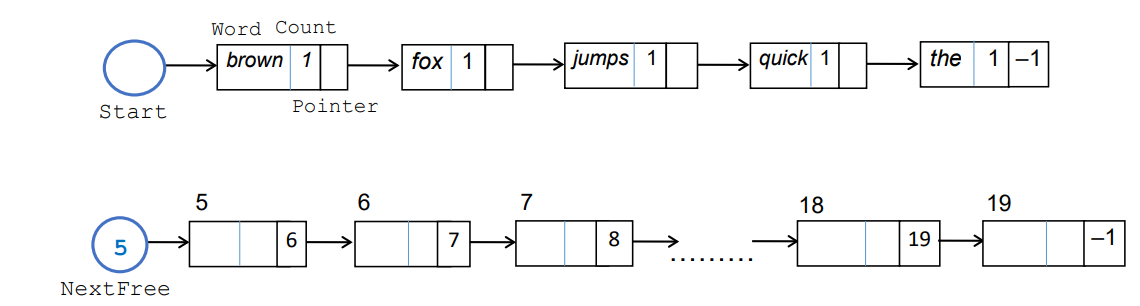
\includegraphics[width=0.7\paperwidth]{C:/Users/Admin/Desktop/Github/question_bank/LyX/static/img/9597-PJC-2018-P1-Q3-1}
\par\end{center}

\subsection*{Task 3.1 }

Write the program code for the classes \texttt{Node} and \texttt{LinkedList},
including the \texttt{Initialise} and \texttt{Display} method. The
code should follow the specifications given. Do not write the \texttt{Insert}
procedure yet.

\subsection*{Evidence 7:}

Your program code for the \texttt{Node} and \texttt{LinkedList} classes.\hfill{}
{[}10{]}

\subsection*{Task 3.2 }

Write program code in the \textbf{main program} to create a linked
list object and display the linked list in index order. 

\subsection*{Evidence 8:}

\textbf{Program code} and \textbf{screenshot} confirming all values
after initialisation of the \texttt{LinkedList} object.\hfill{} {[}3{]}

\subsection*{Task 3.3 }

Write the \texttt{Insert} procedure that will insert a word from the
text into the linked list. If word already exists in linked list,
increment \texttt{Count} by 1.

If word does not exist in linked list, add a new node with the new
word and set \texttt{Count} to 1. You should check for availability
of free node before adding a new node. If you use additional method(s)
and/or variable(s), present them in a table like this: 
\noindent \begin{center}
\begin{tabular}{|c|c|}
\hline 
\textbf{Additional method / variable} & \textbf{Description}\tabularnewline
\hline 
$\cdots$$\cdots$ & $\cdots$$\cdots$$\cdots$$\cdots$\tabularnewline
\hline 
\end{tabular}
\par\end{center}

\textbf{Add appropriate comments to explain your program code.}

\subsection*{Evidence 9: }

Your program code for \texttt{Insert} procedure and other methods
(if any), \textbf{with suitable comments}. Table of additional method(s)
and/or variable(s), if any. \hfill{}{[}17{]}

\subsection*{Task 3.4 }

Write additional code in the \textbf{main program} to read all the
words from the text file \texttt{WORDTEXT.txt} and display the linked
list in index order. 

\subsection*{Evidence 10: }

Your \textbf{additional program code} and \textbf{screenshot} showing
the contents of the linked list after reading in all the words from
the text file \texttt{WORDTEXT.txt}. \hfill{}{[}4{]}

\subsection*{Task 3.5 }

Write a \textbf{recursive} \texttt{ReverseTraversal} procedure that
will traverse the linked list in reverse order and display the words
and its count. 

\subsection*{Evidence 11: }

Your recursive \texttt{ReverseTraversal} \textbf{program code} and
\textbf{screenshot} of running the procedure. \hfill{} {[}6{]}

{[}SPLIT\_HERE{]}
\item \textbf{{[}PJC/PRELIM/9597/2018/P1/Q4{]} }

Records of songs are stored in a hash table. Each song record is an
instance of the class \texttt{SongRecord}, which has \texttt{SongID}
and \texttt{SongTitle} as its data members.

Implement the hash table as an instance of the class \texttt{HashTable}
using the following properties and methods: 
\begin{itemize}
\item Properties
\begin{itemize}
\item \texttt{Size} Maximum number of addresses in hash table 
\item \texttt{Array} One-dimensional array of hash table to store records
indexed \texttt{0} to \texttt{(Size \textendash{} 1)}
\end{itemize}
\item Methods 
\begin{itemize}
\item \texttt{Initialise :} Initialises \texttt{Size} and \texttt{Array}. 
\item \texttt{Hash} 
\begin{itemize}
\item Function to calculate the address of the hash table 
\item Takes \texttt{SongID} as argument
\item ASCII code is calculated for each character from \texttt{SongID}
\item Total of all ASCII values is calculated
\item Total is divided by \texttt{Size} and the remainder calculated with
modulo arithmetic, where \texttt{Size} is the maximum number of locations 
\item Value returned by the function is \texttt{remainder}. This value is
the address for the record in the hash table
\end{itemize}
\item \texttt{Display} 
\begin{itemize}
\item Displays the contents of the hash table under this heading: 
\noindent \begin{center}
\begin{tabular}{|c|c|c|}
\hline 
\texttt{Index} & \texttt{Song ID} & \texttt{Song Title}\tabularnewline
\hline 
$\dots$ & $\dots$ & $\dots$\tabularnewline
\hline 
\end{tabular}
\par\end{center}
\end{itemize}
\item \texttt{Add} 
\begin{itemize}
\item Adds a record into the hash table 
\item Takes \texttt{SongID} and \texttt{SongTitle} as arguments 
\end{itemize}
\item \texttt{Remove} 
\begin{itemize}
\item Removes a record from the hash table
\item Takes \texttt{SongID} as argument 
\end{itemize}
\end{itemize}
\end{itemize}
For example, if \texttt{Size} has value of \texttt{13}, a song record
with \texttt{SongID \textquotedblleft T3311\textquotedblright{}} will
be hashed to address \texttt{11}. 

Total ASCII (\textquotedblleft \texttt{T}\textquotedblright{} + \textquotedblleft \texttt{3}\textquotedblright{}
+ \textquotedblleft \texttt{3}\textquotedblright{} + \textquotedblleft \texttt{1}\textquotedblright{}
+ \textquotedblleft \texttt{1}\textquotedblright ) = 284

284 mod 13 = 11 

Therefore, add record with \texttt{SongID \textquotedblleft T3311\textquotedblright{}}
to the hash table array with address \texttt{11}. 

\subsection*{Task 4.1 }

Write program code for the class \texttt{SongRecord}, with data type
specified clearly for its data members. 

\subsection*{Evidence 12: }

Program code for class \texttt{SongRecord}. \hfill{}{[}4{]}

\subsection*{Task 4.2 }

Write program code for the class \texttt{HashTable}, using the specifications
above. Include all the methods stated: \texttt{Initialise}, \texttt{Hash},
\texttt{Display}, \texttt{Add}, and \texttt{Remove}. 

Assume no collision of records for \texttt{Add} and \texttt{Remove}
here. 

\subsection*{Evidence 13: }

Program code for class \texttt{HashTable}. \hfill{}{[}14{]}

\subsection*{Task 4.3}

Test your program code for \texttt{Size} of value 13, by
\begin{enumerate}
\item \textbf{adding} the following records into the hash table and \textbf{display}
the hash table. You may copy and paste these song records from the
data file \texttt{SONG1.txt}. 

\noindent %
\noindent\begin{minipage}[t]{1\columnwidth}%
\textbf{\uline{Song ID}}\textbf{ ~~~~}\textbf{\uline{Song
Title}}\textbf{ }

\texttt{T3311 ~~Titanium}

\texttt{V2233 ~~Victory }

\texttt{H7444 ~~Happy }

\texttt{G5955 ~~Golden }%
\end{minipage}
\item \textbf{removing} song record \texttt{H7444} and \textbf{display}
the hash table. 
\end{enumerate}

\subsection*{Evidence 14: }

Screenshots of running \textbf{task 4.3 (a) and (b)}.\hfill{} {[}2{]}

\subsection*{Task 4.4 }

Amend your program code to your \texttt{HashTable} class to handle
collisions when more than one record is hashed to the same location.

Explain how the collision handling works. 

\textbf{\emph{When adding a new record}}, ensure that no record with
the same \texttt{SongID} is stored in more than one location. Output
an appropriate message if an existing song record is added. 

\textbf{\emph{When removing a record}}, output an appropriate message
if record does not exist in hash table. 

\subsection*{Evidence 15: }

Amended program code for \texttt{HashTable} class.

Highlight your amended program code in \textbf{bold}. 

Explanation of how collision handling works.\hfill{} {[}8{]}

\subsection*{Task 4.5}

Test your amended program code by 
\begin{enumerate}
\item adding the following song records into the hash table. You may copy
and paste these song records from the data file \texttt{SONG2.txt}. 

\noindent\begin{minipage}[t]{1\columnwidth}%
\textbf{\uline{Song ID}}\textbf{ ~~~~}\textbf{\uline{Song
Title}}

\texttt{G5955 ~~Golden}

\texttt{C9999 ~~Champion }

\texttt{D7474 ~~Delta }

\texttt{J8868 ~~Jump }

\texttt{R1711 ~~Radar} %
\end{minipage}
\item removing song record \texttt{S1234} and \texttt{G5955}.
\end{enumerate}

\subsection*{Evidence 16: }

Screenshots of running \textbf{task 4.5 (a) and (b)}.\hfill{} {[}2{]}

{[}SPLIT\_HERE{]}
\item \textbf{{[}PJC/PRELIM/9597/2018/P1/Q1{]} }

\noindent A Foreign Government Agency is looking for a Tourist Information
Management System. The system should be able to cater for the following
two requirements: 
\begin{enumerate}
\item[a)]  Capture and provision of information for migration control propose
and other aspects of citizen identification 

This is to facilitate the processing of Disembarkation/ Embarkation
(D/E) cards collected from visitors at the checkpoints. It also captures
visitors\textquoteright{} arrival data e.g., the number of arrivals
by countries of residence, their modes of arrival and demographics
(e.g., age and gender). 
\item[b)]  Data Warehouse for analysis 

The Data Warehouse has to receive data and code information on Disembarkation/Embarkation
cards (D/E cards). Information gathered in this manner is to analyse
visitor arrival trends and serve as input to the computation of key
performance indicators (Tourism Receipts, TourismSector Value, etc.)
\end{enumerate}
The Agency wishes to replace this manual system with a computerised
system.

\noindent A system developer is employed to carry out the task. The
first task assigned to the system developer is to write a project
proposal.

One section of the project proposal is the Problem Statement which
lists the problems in the current system. Write the Problem Statement.\hfill{}
{[}6{]}

{[}SPLIT\_HERE{]}
\item \textbf{{[}PJC/PRELIM/9597/2018/P1/Q2{]} }

\noindent A Foreign Government Agency is looking for a Tourist Information
Management System. The system should be able to cater for the following
two requirements: 
\begin{enumerate}
\item[a)]  Capture and provision of information for migration control propose
and other aspects of citizen identification 

This is to facilitate the processing of Disembarkation/ Embarkation
(D/E) cards collected from visitors at the checkpoints. It also captures
visitors\textquoteright{} arrival data e.g., the number of arrivals
by countries of residence, their modes of arrival and demographics
(e.g., age and gender). 
\item[b)]  Data Warehouse for analysis 

The Data Warehouse has to receive data and code information on Disembarkation/Embarkation
cards (D/E cards). Information gathered in this manner is to analyse
visitor arrival trends and serve as input to the computation of key
performance indicators (Tourism Receipts, TourismSector Value, etc.)
\end{enumerate}
The Agency wishes to replace this manual system with a computerised
system.

\noindent A system developer is employed to carry out the task. The
first task assigned to the system developer is to write a project
proposal.

The system developer has drawn up a list of activities and their likely
duration. 
\noindent \begin{center}
\begin{tabular}{|c|c|c|}
\hline 
\textbf{Activity} & \textbf{Description} & \textbf{Weeks to complete}\tabularnewline
\hline 
A & Write requirement specification & 1\tabularnewline
\hline 
B & Produce program design & 1\tabularnewline
\hline 
C & Write module code & 7\tabularnewline
\hline 
D & Module testing & 2\tabularnewline
\hline 
E & Integration testing & 2\tabularnewline
\hline 
F & Alpha testing & 2\tabularnewline
\hline 
G & Install software and carry out acceptance testing & 2\tabularnewline
\hline 
H & Research and order hardware & 1\tabularnewline
\hline 
J & Install delivered hardware & 3\tabularnewline
\hline 
K & Write technical documentation & 4\tabularnewline
\hline 
L & Write user training guide & 2\tabularnewline
\hline 
M & Train users on installed hardware and software & 1\tabularnewline
\hline 
N & Sign off final system & 1\tabularnewline
\hline 
\end{tabular}
\par\end{center}
\begin{enumerate}
\item From this data a GANTT chart is constructed. \hfill{}{[}2{]}
\noindent \begin{center}
\begin{tabular}{|c|c|c|c|c|c|c|c|c|c|c|c|c|c|c|c|c|c|c|c|c|c|c|c|c|c|c|c|}
\hline 
\textbf{Activity} & X &  &  &  &  &  &  &  &  &  &  &  &  &  &  &  &  &  &  &  &  &  &  &  &  &  & \tabularnewline
\hline 
A & X &  &  &  &  &  &  &  &  &  &  &  &  &  &  &  &  &  &  &  &  &  &  &  &  &  & \tabularnewline
\hline 
B &  & X &  &  &  &  &  &  &  &  &  &  &  &  &  &  &  &  &  &  &  &  &  &  &  &  & \tabularnewline
\hline 
C &  &  & X & X & X & X & X & X & X &  &  &  &  &  &  &  &  &  &  &  &  &  &  &  &  &  & \tabularnewline
\hline 
D &  &  &  &  &  &  &  &  & X & X &  &  &  &  &  &  &  &  &  &  &  &  &  &  &  &  & \tabularnewline
\hline 
E &  &  &  &  &  &  &  &  &  &  & X & X &  &  &  &  &  &  &  &  &  &  &  &  &  &  & \tabularnewline
\hline 
F &  &  &  &  &  &  &  &  &  &  &  &  & X & X &  &  &  &  &  &  &  &  &  &  &  &  & \tabularnewline
\hline 
G &  &  &  &  &  &  &  &  &  &  &  &  &  &  & X & X &  &  &  &  &  &  &  &  &  &  & \tabularnewline
\hline 
H &  &  & X &  &  &  &  &  &  &  &  &  &  &  &  &  &  &  &  &  &  &  &  &  &  &  & \tabularnewline
\hline 
J &  &  &  & X & X & X &  &  &  &  &  &  &  &  &  &  &  &  &  &  &  &  &  &  &  &  & \tabularnewline
\hline 
K &  &  &  &  &  &  &  &  &  &  & X & X & X & X &  &  &  &  &  &  &  &  &  &  &  &  & \tabularnewline
\hline 
L &  &  &  &  &  &  &  &  &  &  &  &  &  &  & X & X &  &  &  &  &  &  &  &  &  &  & \tabularnewline
\hline 
M &  &  &  &  &  &  &  &  &  &  &  &  &  &  &  &  &  &  &  &  &  &  &  &  &  &  & \tabularnewline
\hline 
N &  &  &  &  &  &  &  &  &  &  &  &  &  &  &  &  &  &  &  &  &  &  &  &  &  &  & \tabularnewline
\hline 
Week Number & 1 & 2 & 3 & 4 & 5 & 6 & 7 & 8 & 9 & 10 & 11 & 12 & 13 & 14 & 15 & 16 & 17 & 18 & 19 & 20 & 21 & 22 & 23 & 24 & 25 & 26 & 27\tabularnewline
\hline 
\end{tabular}
\par\end{center}
\item State the earliest completion date in terms of week number.\hfill{}
{[}1{]}
\item There are problems with the progress of the project: 
\begin{itemize}
\item Activity E showed that the code contained major errors. The senior
programmer now estimates that:
\begin{itemize}
\item further module coding will require another 2 weeks
\item further module testing will require another 2 weeks 
\item further integration testing will require another 2 weeks 
\end{itemize}
\item The hardware delivery is delayed by 16 weeks 
\end{itemize}
A revised GANTT chart is now required 

Copy and complete the chart in the grid below
\noindent \begin{center}
\begin{tabular}{|c|c|c|c|c|c|c|c|c|c|c|c|c|c|c|c|c|c|c|c|c|c|c|c|c|c|c|c|}
\hline 
\textbf{Activity} & X &  &  &  &  &  &  &  &  &  &  &  &  &  &  &  &  &  &  &  &  &  &  &  &  &  & \tabularnewline
\hline 
A & X &  &  &  &  &  &  &  &  &  &  &  &  &  &  &  &  &  &  &  &  &  &  &  &  &  & \tabularnewline
\hline 
B &  & X &  &  &  &  &  &  &  &  &  &  &  &  &  &  &  &  &  &  &  &  &  &  &  &  & \tabularnewline
\hline 
C &  &  & X & X & X & X & X & X & X &  &  &  &  &  &  &  &  &  &  &  &  &  &  &  &  &  & \tabularnewline
\hline 
D &  &  &  &  &  &  &  &  & X & X &  &  &  &  &  &  &  &  &  &  &  &  &  &  &  &  & \tabularnewline
\hline 
E &  &  &  &  &  &  &  &  &  &  & X & X &  &  &  &  &  &  &  &  &  &  &  &  &  &  & \tabularnewline
\hline 
F &  &  &  &  &  &  &  &  &  &  &  &  &  &  &  &  &  &  &  &  &  &  &  &  &  &  & \tabularnewline
\hline 
G &  &  &  &  &  &  &  &  &  &  &  &  &  &  &  & X &  &  &  &  &  &  &  &  &  &  & \tabularnewline
\hline 
H &  &  & X &  &  &  &  &  &  &  &  &  &  &  &  &  &  &  &  &  &  &  &  &  &  &  & \tabularnewline
\hline 
J &  &  &  &  &  &  &  &  &  &  &  &  &  &  &  &  &  &  &  &  &  &  &  &  &  &  & \tabularnewline
\hline 
K &  &  &  &  &  &  &  &  &  &  &  &  &  &  &  &  &  &  &  &  &  &  &  &  &  &  & \tabularnewline
\hline 
L &  &  &  &  &  &  &  &  &  &  &  &  &  &  &  &  &  &  &  &  &  &  &  &  &  &  & \tabularnewline
\hline 
M &  &  &  &  &  &  &  &  &  &  &  &  &  &  &  &  &  &  &  &  &  &  &  &  &  &  & \tabularnewline
\hline 
N &  &  &  &  &  &  &  &  &  &  &  &  &  &  &  &  &  &  &  &  &  &  &  &  &  &  & \tabularnewline
\hline 
Week Number & 1 & 2 & 3 & 4 & 5 & 6 & 7 & 8 & 9 & 10 & 11 & 12 & 13 & 14 & 15 & 16 & 17 & 18 & 19 & 20 & 21 & 22 & 23 & 24 & 25 & 26 & 27\tabularnewline
\hline 
\end{tabular}
\par\end{center}

\hfill{}{[}9{]}
\item State the new estimated completion date in terms of week number. \hfill{}{[}1{]}
\end{enumerate}
A team was formed for the designing of this project. 
\begin{enumerate}
\item[(e)]  Why the team work and the roles of team members working on a computer
project are important? \hfill{}{[}2{]}
\end{enumerate}
{[}SPLIT\_HERE{]}
\item \textbf{{[}PJC/PRELIM/9597/2018/P1/Q3{]} }

\noindent A Foreign Government Agency is looking for a Tourist Information
Management System. The system should be able to cater for the following
two requirements: 
\begin{enumerate}
\item[a)]  Capture and provision of information for migration control propose
and other aspects of citizen identification 

This is to facilitate the processing of Disembarkation/ Embarkation
(D/E) cards collected from visitors at the checkpoints. It also captures
visitors\textquoteright{} arrival data e.g., the number of arrivals
by countries of residence, their modes of arrival and demographics
(e.g., age and gender). 
\item[b)]  Data Warehouse for analysis 

The Data Warehouse has to receive data and code information on Disembarkation/Embarkation
cards (D/E cards). Information gathered in this manner is to analyse
visitor arrival trends and serve as input to the computation of key
performance indicators (Tourism Receipts, TourismSector Value, etc.)
\end{enumerate}
The Agency wishes to replace this manual system with a computerised
system.

The design for the new system includes the provision of a network
of computers in the office with a central file server. Each office
staff will have access to a computer to retrieve and update visitors\textquoteright{}
data held on the central file server. Some support staff are allowed
to access the data but not change it. In addition the system has an
Internet link which allows staff to access the system from outside
the office. 

Describe \textbf{three} ways in which the security of this system
can be implemented. \hfill{}{[}3{]}

{[}SPLIT\_HERE{]}
\item \textbf{{[}PJC/PRELIM/9597/2018/P1/Q4{]} }

\noindent A Foreign Government Agency is looking for a Tourist Information
Management System. The system should be able to cater for the following
two requirements: 
\begin{enumerate}
\item[a)]  Capture and provision of information for migration control propose
and other aspects of citizen identification 

This is to facilitate the processing of Disembarkation/ Embarkation
(D/E) cards collected from visitors at the checkpoints. It also captures
visitors\textquoteright{} arrival data e.g., the number of arrivals
by countries of residence, their modes of arrival and demographics
(e.g., age and gender). 
\item[b)]  Data Warehouse for analysis 

The Data Warehouse has to receive data and code information on Disembarkation/Embarkation
cards (D/E cards). Information gathered in this manner is to analyse
visitor arrival trends and serve as input to the computation of key
performance indicators (Tourism Receipts, TourismSector Value, etc.)
\end{enumerate}
The Agency wishes to replace this manual system with a computerised
system.

The office staff enters information provided by visitor into the computer
system using a graphical user interface. Some of the information required
includes: 
\begin{itemize}
\item Passport number 
\item visitor\textquoteright s salutation (e.g. Dr., Mr., Ms, Mrs, Mdm\dots ) 
\item visitor name and address 
\item visitor gender (e.g. F or M)
\item mobile number 
\end{itemize}
For this application design a simple screen layout which makes use
of appropriate graphical user interface controls. \hfill{}{[}3{]}

{[}SPLIT\_HERE{]}
\item \textbf{{[}PJC/PRELIM/9597/2018/P1/Q5{]} }

Top-down design is a technique used to produce solutions to computer
system. 
\begin{enumerate}
\item Explain the term top-down design. \hfill{}{[}3{]}
\item Explain \textbf{three} advantages of using top-down design to solve
complex problems.\hfill{} {[}3{]}
\item Explain \textbf{three} techniques that can be used to ensure that
program code is understandable and can be easily maintained. \hfill{}{[}3{]}
\end{enumerate}
{[}SPLIT\_HERE{]}
\item \textbf{{[}PJC/PRELIM/9597/2018/P1/Q6{]} }

The following pseudo-code algorithm describes one method of finding
an arbitrary visitor name in an alphabetically ordered array of N
unique names. 

\noindent %
\noindent\begin{minipage}[t]{1\columnwidth}%
set first to 1 

set last to N 

repeat 

\texttt{\qquad{}}set mid to the integer part of (first + last) /2 

\texttt{\qquad{}}If the mid name precedes the wanted name then 

\texttt{\qquad{}\qquad{}}set first to mid + 1 

\texttt{\qquad{}}else 

\texttt{\qquad{}\qquad{}}set last to mid - 1

\texttt{\qquad{}}endif 

until first > last or midth name is the wanted name%
\end{minipage}
\begin{enumerate}
\item If 142 names are stored in the array, and JOSEPH is the 44th name,
state the elements of the array that are examined when searching for
JOSEPH. \hfill{}{[}4{]}
\item If a search is made for a name that is not in the array, what is the
largest number of elements that might need to be examined before one
could say that the name is not present? Explain how you arrive at
your answer. \hfill{}{[}3{]}
\end{enumerate}
{[}SPLIT\_HERE{]}
\item \textbf{{[}PJC/PRELIM/9597/2018/P1/Q7{]} }

Visitors can claim the GST (Goods and Services Tax) before they leave
the country. A programmer is going to write part of the computer system
using an object-oriented programming (OOP) language, which will store
details of claims by visitor either pay by cash or hand phone transfer.
The claim receive by hand phone transfer will have a rebate of 0.2\%.
while claim receive by cash will have to pay 0.5\% of service charge
and recording the currency exchange rate. 

Properties identified the claims included: 
\begin{itemize}
\item Passport number
\item Receipt number 
\end{itemize}
Type of claims (cash or hand phone transfer)
\begin{enumerate}
\item Draw a diagram that shows how the properties could be distributed
amongst a number of classes. Include in your diagram any inheritance
between classes. Also indicate appropriate methods (including one
pair of 'get' and 'set' methods for one of the properties) that would
be required. One method should demonstrate polymorphism. {[}6{]}
\item In the context of object-oriented programming explain what is meant
by: 
\begin{enumerate}
\item Encapsulation and how classes support information hiding and implementation
independence. \hfill{} {[}3{]}
\item Inheritance and how it promotes software reuse. \hfill{}{[}2{]}
\item Polymorphism and how it enables code generalisation. \hfill{}{[}2{]}
\item Computational thinking and why it is important? \hfill{} {[}5{]}
\end{enumerate}
\item Give \textbf{two} advantages of object-oriented programming. \hfill{}{[}2{]}
\end{enumerate}
{[}SPLIT\_HERE{]}
\item \textbf{{[}PJC/PRELIM/9597/2018/P1/Q8{]} }

The system developer recommending cloud computing for the Agency. 
\begin{enumerate}
\item What are the \textbf{three} different layers of cloud computing? \hfill{}{[}3{]}
\item Discuss the benefits and drawbacks of using the cloud for storing
data rather than other methods. \hfill{} {[}4{]}
\end{enumerate}
{[}SPLIT\_HERE{]}
\item \textbf{{[}PJC/PRELIM/9597/2018/P1/Q9{]} }

PJ Mall plans to create a database to store data on its shops. It
rents out shops to tenants who run their business.
\begin{itemize}
\item Each \emph{tenant} is to provide information on its \emph{company
name}, \emph{director of company}, \emph{company address}, \emph{contact
number}, and \emph{retail type}. 
\item There is a \emph{start} and \emph{end} date for every rental.
\item Each \emph{shop} rented by the tenant consists of one or more unit
spaces. 
\item Each unit space is located at a particular \emph{level} and has a\emph{
unit number}. 
\item There are 3 categories of unit space. Each \emph{category} has its
own \emph{size} and \emph{rental rate}. 
\noindent \begin{center}
\begin{tabular}{|c|c|c|}
\hline 
Category & Size (square feet) & Rental rate (\$ per square feet)\tabularnewline
\hline 
A & Less than 200 & 40\tabularnewline
\hline 
B & 200 -- 2000 & 30\tabularnewline
\hline 
C & More than 2000 & 20\tabularnewline
\hline 
\end{tabular} 
\par\end{center}

\end{itemize}
Here are some tenants who run their business in PJ mall: 
\noindent \begin{center}
\begin{tabular}{|c|c|c|c|}
\hline 
Company Name & Level & Unit Number & Retail Type\tabularnewline
\hline 
Bata & 2 & 03 -- 04 & Footwear\tabularnewline
\hline 
Challenger & 2 & 06 -- 08 & Technology\tabularnewline
\hline 
Coldwear & 3 & 08 & Fashion\tabularnewline
\hline 
Esprit & 3 & 09 -- 10 & Fashion\tabularnewline
\hline 
Giant & 1 & 01 -- 12 & Supermarket\tabularnewline
\hline 
Hi Tea & 1 & 14 & Food \& Beverage\tabularnewline
\hline 
PappaRich & 2 & 11 -- 13 & Food \& Beverage\tabularnewline
\hline 
$\dots$ & $\dots$ & $\dots$ & $\dots$\tabularnewline
\hline 
\end{tabular}
\par\end{center}
\begin{enumerate}
\item A solution is to create a relational database which requires a number
of tables to store data for this application. 
\begin{enumerate}
\item Draw the E-R diagram showing the tables and the relationships between
them. \hfill{} {[}5{]}
\item A table description can be described as 

\texttt{TableName(Attribute1, Attribute2, Attribute3, \dots \dots ) }

The primary key is indicated by underlining one or more attributes.
Write table descriptions for the tables in part \textbf{(i)}. \hfill{}
{[}6{]}
\end{enumerate}
\item Describe \textbf{two} advantages of using a relational database for
storing data on its shops rather than a customised software. \hfill{}
{[}4{]}
\end{enumerate}
{[}SPLIT\_HERE{]}
\item \textbf{{[}PJC/PRELIM/9597/2018/P1/Q10{]} }

A dataset of fruit names is to be stored in a binary search tree. 

The names of the fruits are inserted into the tree in the order shown: 
\noindent \begin{center}
\texttt{Papaya, Mango, Durian, Strawberry, Orange, Rambutan, Watermelon}
\par\end{center}
\begin{enumerate}
\item Draw the binary search tree. \hfill{} {[}3{]}
\end{enumerate}
The binary tree is implemented using these identifiers. 
\noindent \begin{center}
\begin{tabular}{|c|c|c|}
\hline 
\textbf{Variable} & \textbf{Data Type} & \textbf{Description}\tabularnewline
\hline 
\texttt{RootPtr} & \texttt{INTEGER} & Array subscript of the root of tree\tabularnewline
\hline 
\texttt{Fruit} & \texttt{ARRAY {[}1..100{]} of STRING} & Array of fruit names\tabularnewline
\hline 
\texttt{LeftPtr} & \texttt{ARRAY {[}1..100{]} of INTEGER} & Array of left pointer values\tabularnewline
\hline 
\texttt{RightPtr} & \texttt{ARRAY {[}1..100{]} of INTEGER} & Array of right pointer values \tabularnewline
\hline 
\end{tabular}
\par\end{center}
\begin{enumerate}
\item[(b)]  Draw a diagram to show the contents of the binary tree in array
form and the root pointer variable for the fruits inserted in \textbf{(a)}
above. \hfill{}{[}3{]}
\item[(c)]  The pseudocode shows an algorithm to search for a particular fruit
in the binary tree. Additional variables \texttt{SearchFruit}, \texttt{IsFound},
and \texttt{Current} are used. 

\noindent\fbox{\begin{minipage}[t]{1\columnwidth - 2\fboxsep - 2\fboxrule}%
\texttt{\textbf{INPUT}}\texttt{ SearchFruit }

\texttt{IsFound \textleftarrow{} False }

\texttt{Current \textleftarrow{} RootPtr }

\texttt{\textbf{REPEAT}}\texttt{ }

\texttt{\qquad{}}%
\fbox{\begin{minipage}[t]{0.4\columnwidth}%

\subsubsection*{\texttt{... ... ...}}

\subsubsection*{\texttt{... ... ...}}

\subsubsection*{\texttt{... ... ...}}%
\end{minipage}}

\texttt{\textbf{UNTIL}}\texttt{ Current = 0 }\texttt{\textbf{OR}}\texttt{
IsFound = }\texttt{\textbf{TRUE}}\texttt{ }

\texttt{\textbf{IF}}\texttt{ IsFound = False }\texttt{\textbf{THEN}}\texttt{ }

\texttt{\qquad{}}\texttt{\textbf{OUTPUT}}\texttt{ SearchFruit \textquotedbl Not
found\textquotedbl{} }

\texttt{\textbf{ENDIF}}\texttt{ }%
\end{minipage}}

Complete the algorithm in the \texttt{\textbf{REPEAT-UNTIL}} loop
by writing the missing lines. \hfill{}{[}6{]}
\end{enumerate}
{[}SPLIT\_HERE{]}
\item \textbf{{[}PJC/PRELIM/9597/2018/P1/Q11{]} }

The ASCII encoding system can be used to represent characters on computers. 
\begin{enumerate}
\item The ASCII code in decimal for the numeric character \textquoteleft 1\textquoteright{}
is 49. Using 8 bits, what is the ASCII code for the character \textquoteleft 4\textquoteright{}
in binary? \hfill{}{[}2{]}
\item The ASCII codes for uppercase letters are from \texttt{01000001} for
\textquoteleft A\textquoteright{} to \texttt{01011010} for \textquoteleft Z\textquoteright .
What is the ASCII code for \textquoteleft W\textquoteright{} in binary?
\hfill{}{[}2{]}
\item An alternative encoding system is Unicode. State \textbf{one} advantage
and \textbf{one} disadvantage of using ASCII rather than Unicode.
\hfill{} {[}2{]}
\end{enumerate}
{[}SPLIT\_HERE{]}
\item \textbf{{[}PJC/PRELIM/9597/2018/P1/Q12{]} }

A fashion shop gives customers a discount on purchases totalling more
than \$30: 
\begin{itemize}
\item Discount of 5\% with a member card 
\item Discount of 5\% for purchases totalling more than \$200 
\item Discount of 10\% with a member card and for purchases totalling more
than \$200
\end{itemize}
Draw a decision table and simplify it by removing redundancies. \hfill{}
{[}8{]}

{[}SPLIT\_HERE{]}
\item \textbf{{[}PJC/PRELIM/9597/2018/P1/Q13{]} }

The following list of numbers is to be sorted in ascending order. 
\noindent \begin{center}
\texttt{98, 12, 23, 8, 74, 30, 62 }
\par\end{center}
\begin{enumerate}
\item Show the list of numbers \textbf{after each pass} by performing
\begin{enumerate}
\item a bubble sort, \hfill{}{[}3{]}
\item an insertion sort. \hfill{}{[}3{]}
\end{enumerate}
\item By comparing how the bubble and insertion sort work, explain which
one is a faster sort. \hfill{}{[}3{]}
\end{enumerate}
{[}SPLIT\_HERE{]}
\end{enumerate}

\end{document}
